\chapter{Exact solution for Lens Models}

\section{Axially-Symmetric Models}

\subsection{SIS}
The most single lens model for galaxies  corresponds to Singular Isothermal
Sphere. This model, is obtained by assuming a spherical mass distribution
that behaves as an isothermal gas in hidrostatic equilibrium. In this case,
the density is given by

\begin{equation}
 \rho(r)=\dfrac{\sigma_v^2}{2\pi G r^2},
\end{equation}
where $\sigma_v$ is the peculiar velocity  and $r=\sqrt{\xi^2+z^2}$ is the
distance to the center of the sphere. 

Choosing $\xi_0= \dfrac{4\pi \sigma^2_v D_{\rm LS} D_{\rm OS}}{c^2 D_{\rm
OS}}$ for the dimensionless coordinates $\vec{x}=\frac{\vec{\xi}}{\xi_0}$, the
lensing potential is given by

\begin{equation}
 \varphi(x)=x,
\label{sis_pot}
\end{equation}
where $x=\sqrt{x^2_1+x^2_2}$. From the lensing potential above, the lensing
functions are
\begin{eqnarray}
 \alpha(\vec{x}) &=& 1 \label{sis_angle}\\
\kappa(\vec{x}) &= & \dfrac{1}{2x} \label{sis_convg}\\
\gamma(\vec{x}) & = &  \dfrac{1}{2x} \label{sis_shear}.
\end{eqnarray}
Notice that, the vectorial expression for the deflection angle,
Eq.~(\ref{sis_angle}), is
\begin{equation}
 \vec{\alpha}(\vec{x})=\cos{\phi}\hat{\imath} + \sin{\phi}\hat{\jmath},
\end{equation}
where $\phi=\arctan{(x_2/x_1)}$


\section{Pseudo-Elliptical Models}
To distort a circular lensing potential $\varphi(x)$ into a elliptical shape $\varphi_\varepsilon(x)$, its radial
coordinate $x$ is replaced by $x_\varepsilon$, where $x_\varepsilon$ is given 
\begin{equation}
 x \rightarrow x_\varepsilon = \sqrt{x^2_{1\varepsilon}+x^2_{2\varepsilon}}=
\sqrt{a_{1\varepsilon}\,x^2_1+a_{2\varepsilon}\,x^2_2}.%
\label{subti-ellip}
\end{equation}

\noindent In general, for any choice of $a_{1\varepsilon}$ and
$a_{2\varepsilon}$, the lensing functions have simple analytical expressions.
For example, the angle deflection, convergence and the components of the
shear are 
\begin{eqnarray}
\vec{\alpha}_\varepsilon(\vec{x})&=&\alpha(x_\varepsilon)(\sqrt{a_{1\varepsilon}
} \cos { \phi_ \varepsilon},\sqrt{a_{2\varepsilon}}\sin{\phi_\varepsilon})
\label{ang_def_pe}\\
\kappa_\varepsilon(\vec{x})&=&\mathcal{A}(\varepsilon)\kappa(x_\varepsilon)
-\mathcal{B}(\varepsilon)\gamma(x_\varepsilon)\cos{2\phi_\varepsilon}
\label{kappa_pe}\\
\gamma_{1\varepsilon}(\vec{x})& = &
\mathcal{B}(\varepsilon)\kappa(x_\varepsilon)-\mathcal{A}
(\varepsilon)\gamma(x_\varepsilon)\cos{2\phi_\varepsilon} \\
\gamma_{2\varepsilon}(\vec{x})& =
&-\sqrt{\mathcal{A}^2(\varepsilon)-\mathcal{B}^2(\varepsilon)}
\gamma(x_\varepsilon)\sin{ 2\phi_\varepsilon}\\
\gamma^2_\varepsilon(\vec{x}) & = &
\mathcal{A}^2(\varepsilon)\gamma^2(x_\varepsilon)-2\mathcal{A}
(\varepsilon)\mathcal {B}
(\varepsilon)\kappa(x_\varepsilon)\gamma(x_\varepsilon)\cos{2\phi_\varepsilon}
\nonumber  \\ &  &
+\mathcal{B}^2(\varepsilon)[\kappa^2(x_\varepsilon)-\sin^2{2\phi_\varepsilon}
\gamma^2(x_\varepsilon) ]\label{gamma_pe}
\end{eqnarray}
\noindent where
$\phi_\varepsilon=\arctan(\frac{x_{2\varepsilon}}{x_{1\varepsilon}})$,
$\mathcal{A(\varepsilon)}=\frac{1}{2}(a_{1\varepsilon}+a_{2\varepsilon})$ and
$\mathcal{B}(\varepsilon)=\frac{1}{2}(a_{1\varepsilon}-a_{2\varepsilon})$.
$\kappa(x_\varepsilon)$
and $\gamma(x_\varepsilon)$ are respectively the convergence and shear of any
circular model, in
which $x$ was replaced by $x_\varepsilon$.


\subsection{SIEP}
For this kind of model, from Eq.~(\ref{sis_pot}) and Eq.~(\ref{subti-ellip})
the lensing potential reads
\begin{equation}
 \varphi_\varepsilon(\vec{x})=x_\varepsilon,\label{siep_pot}
\end{equation}
 and its lensing functions are
\begin{eqnarray}
\vec{\alpha}_\varepsilon(\vec{x}) & = & (\sqrt{a_{1\varepsilon}
} \cos { \phi_ \varepsilon},\sqrt{a_{2\varepsilon}}\sin{\phi_\varepsilon})\\
\kappa_\varepsilon(\vec{x}) & = &
\left[\mathcal{A}(\varepsilon)-\mathcal{B}(\varepsilon)\cos{2\phi_\varepsilon}
\right](2 x_\varepsilon)^{-1}=\gamma_\varepsilon(\vec{x})
\end{eqnarray}
From the equations above, the components of the lens equation are
\begin{eqnarray}
 y_1&=&\dfrac{x_\varepsilon\cos{\phi_\varepsilon}}{\sqrt{a_{1\varepsilon}}}-\sqrt{a_{1\varepsilon}}\cos{\phi_ \varepsilon} \label{y1_siep}\\
y_2&=&\dfrac{x_\varepsilon\sin{\phi_\varepsilon}}{\sqrt{a_{2\varepsilon}}}-\sqrt{a_{2\varepsilon}}\sin{\phi_ \varepsilon} \label{y2_siep},
\end{eqnarray}
and the expression for the eigenvalues read
\begin{eqnarray}
\lambda_r(\vec{x})&=& 1-\kappa_\varepsilon(\vec{x})+\gamma_\varepsilon(\vec{x} )=1 \label{lr_siep}\\
\lambda_t(\vec{x})& =& 1-\kappa_\varepsilon(\vec{x})-\gamma_\varepsilon(\vec{x}
)=1-\left[\mathcal{A}(\varepsilon)-\mathcal{B}(\varepsilon)\cos{2\phi_\varepsilon } \right](x_\varepsilon)^{-1} \label{lt_siep}
\end{eqnarray}

From the Eq.~(\ref{lr_siep}) since $\lambda_r=1$ is not null, the radial critical curve is degenerated into a point $x_{rcc}=0$, and therefore the components of the radial caustic is
 \begin{eqnarray}
y_{1,rca} &=&-\sqrt{a_{1\varepsilon}}\cos{\phi_ \varepsilon}\\
y_{2,rca} &=&-\sqrt{a_{2\varepsilon}}\sin{\phi_ \varepsilon},
\end{eqnarray}

From the Eq.~(\ref{lt_siep}) the pseudo-elliptical radial coordinate of the tangential critical curve  ($\lambda_t=0$) is
\begin{equation}
x_{\varepsilon,tcc}= \mathcal{A}(\varepsilon)-\mathcal{B}(\varepsilon)\cos{2\phi_\varepsilon}, 
\end{equation}
then, the cartesian coordinates of the tangential critical are
\begin{equation}
x_{1,tcc}=\dfrac{x_{\varepsilon,tcc}\cos{\phi_\varepsilon}}{\sqrt{a_{1\varepsilon}}},\qquad x_{2,tcc}=\dfrac{x_{\varepsilon,tcc}\sin{\phi_\varepsilon}}{\sqrt{a_{2\varepsilon}}},
\end{equation}
and the componente of the tangential caustic are
\begin{eqnarray}
y_{1,tca} &=&x_{1,tcc}-\sqrt{a_{1\varepsilon}}\cos{\phi_\varepsilon}\\
y_{2,tca} &=&x_{2,tcc}-\sqrt{a_{2\varepsilon}}\sin{\phi_\varepsilon},
\end{eqnarray}

Besides, the local approximation for the length-to-width ratio of arcs $R_\lambda:=\lambda_r/\lambda_t$ implies
\begin{equation}
R_{\rm th}=\dfrac{1}{1-\left[\mathcal{A}(\varepsilon)-\mathcal{B}(\varepsilon)\cos{2\phi_\varepsilon } \right](x_\varepsilon)^{-1}},
\end{equation}
and the pseudo-elliptical radial coordinates of the curves of constant distortion (in the lens plane) are
\begin{equation}
x_{\varepsilon,R_{\rm th}}=x_{\varepsilon,tcc}\times\left\{\begin{array}{cc} \dfrac{|R_{\rm th}|}{|R_{\rm th}|-1}, & R_{\rm th}>0 \\ & \\
\dfrac{|R_{\rm th}|}{|R_{\rm th}|+1}, & R_{\rm th}<0 \end{array}\right.
\end{equation}
The cartesian components of the cuves of constant distortion in the source plane are given by the Eqs.~(\ref{y1_siep}) and (\ref{y2_siep}) where $x_\varepsilon$ is replaced by $x_{\varepsilon,R_{\rm th}}$.

In Fig.~\ref{siep_curves} we show an example for the main curves of the SIEP model in both planes, for $R_{\rm E}=1$, $\varepsilon=0.4$ (that corresponds to the lensing potential ellipticity by itself).

\begin{figure*}[!ht]
\resizebox{\hsize}{!}{
\subfigure{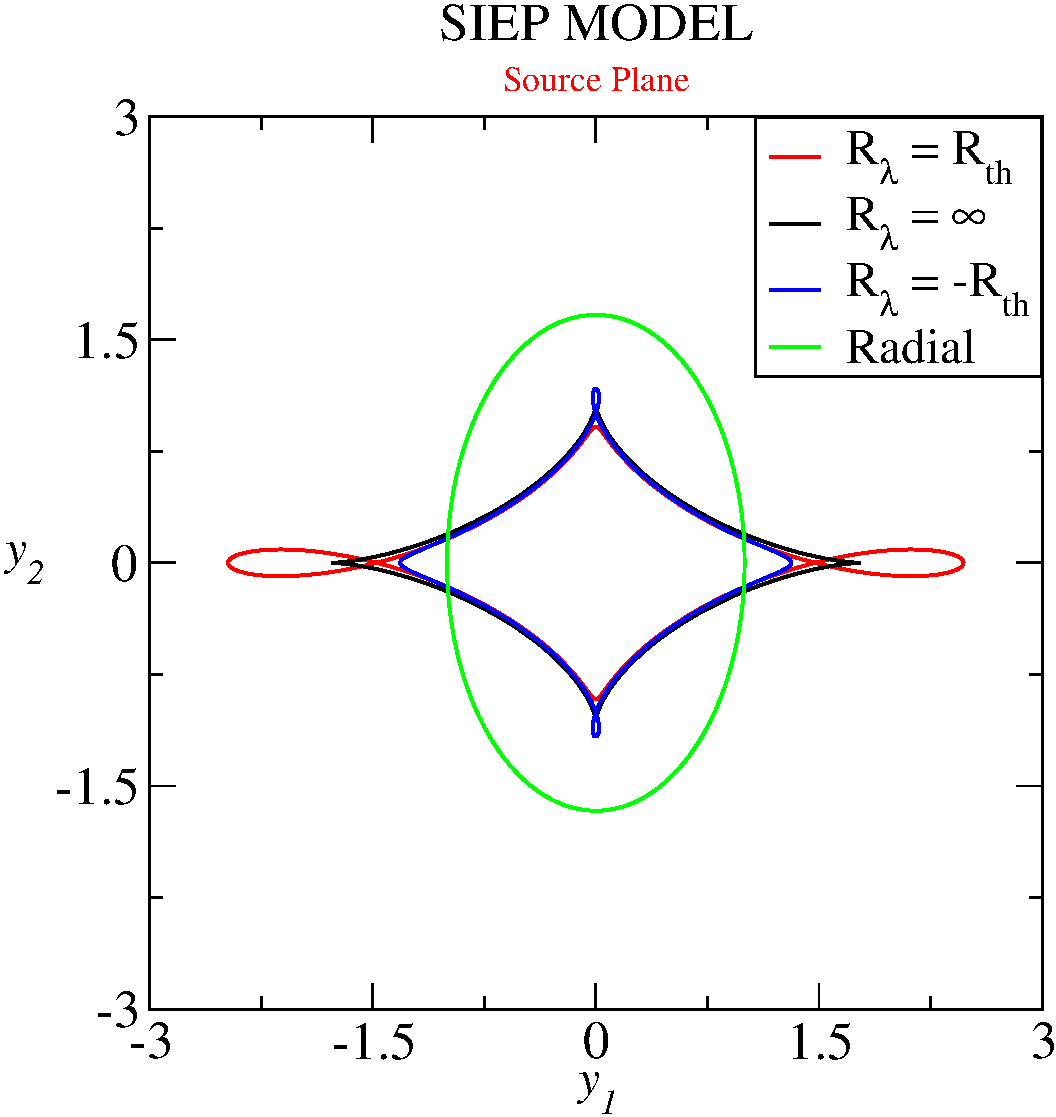
\includegraphics{graphics/siep_source_plane.pdf}}
\hspace{3.cm}
\subfigure{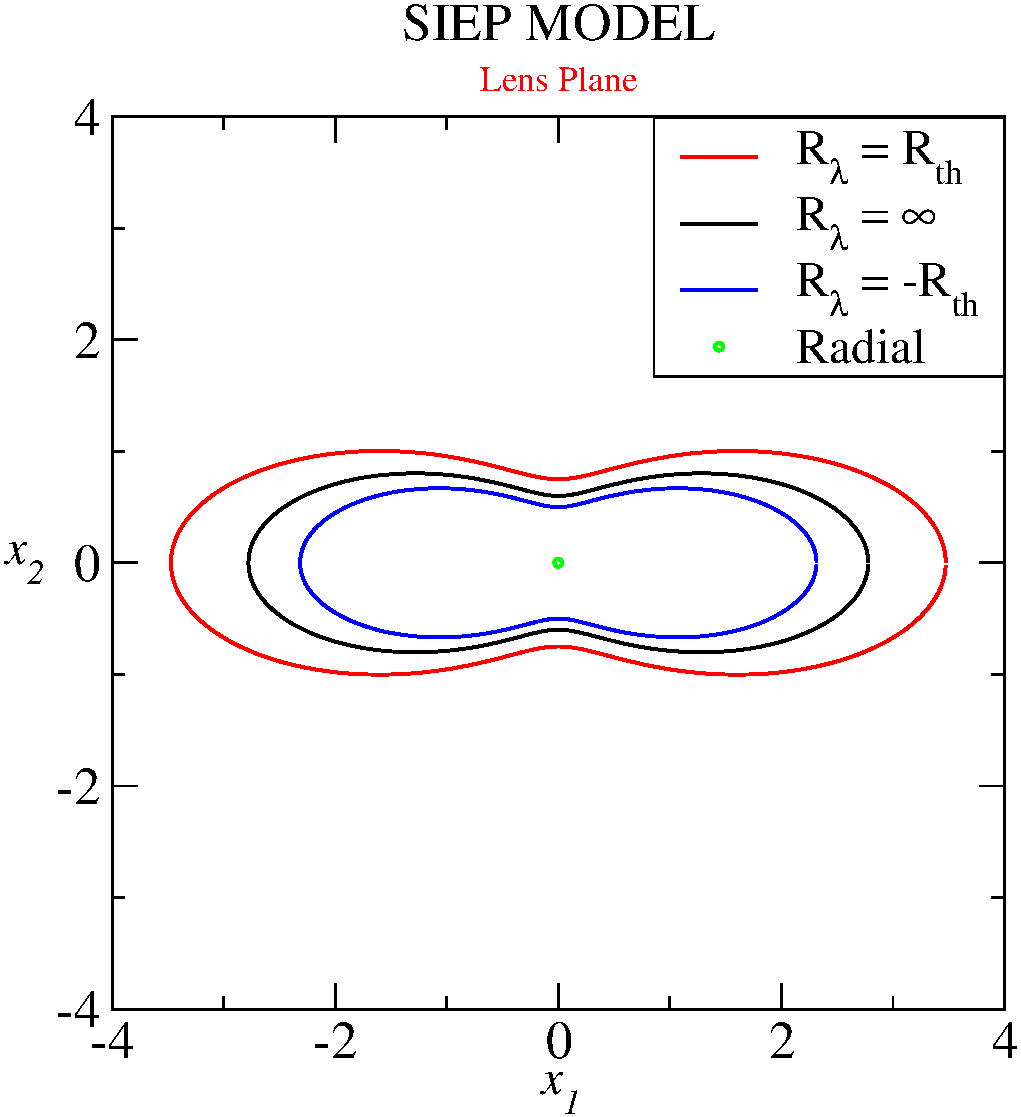
\includegraphics{graphics/siep_lens_plane.pdf}}}
\caption{\label{siep_curves}  SIEP lensing model curves. Left Panel:
Tangential($R_\lambda=\infty$) and Radial Caustics and Curves of Constant
Distortion ($R_\lambda=\pm R_{\rm th}$) . Right Panel: Tangential
($R_\lambda=\infty$) and Radial Critical Curves and  Constant Distortion Curves
($R_\lambda=\pm R_{\rm th}$). Here, we used $R_{\rm E}=1$ and $|R_{\rm
th}|=5$ and the Keeton's parametrization,i.e,  $a_{1\varepsilon}=1$ and
$a_{2\varepsilon}=(1-\varepsilon)^{-2}$ for $\varepsilon=0.4$, }
\end{figure*}

{\bf to be continued\ldots}
\section{Elliptical Models}